\section{Fourierreihe}
  	Komplex: $$\boxed{f(t) = \sum\limits_{k = -\infty}^{\infty} c_k \cdot e^{j k
  	\omega_f t}}= \sum\limits_{k = 0}^{\infty} \left(c_k \cdot e^{j k \omega_f
  	t} + \overline{c_k} \cdot e^{-j k \omega_f t}\right) \quad
  	\boxed{c_k=\overline{c_{-k}}=\frac{1}{T}\int_0^T{f(t)\cdot
	e^{-jk\omega_f t}dt}}$$
	
	\vspace{0.5cm}
	
  	Reell: $$\boxed{f(t) = \frac{a_0}{2} + \sum\limits_{k=1}^{\infty} \left[a_k
  	\cos(k \omega_f t) + b_k \sin(k \omega_f t)\right]}=\frac{A_0}{2} +
  	\sum\limits_{k=1}^{\infty} A_k \cos(k \omega_f t + \varphi_k) \quad k\in
  	\mathbb{Z}$$	
	
	$$\boxed{a_0 =
	\frac{2}{T}\int\limits_0^{T} f(t)dt, \quad a_k = \frac{2}{T}\int\limits_0^{T} f(t)\cos(k \omega_f t) dt, \quad b_k =
	\frac{2}{T}\int\limits_0^{T} f(t)\sin(k \omega_f t) dt} \quad
	\boxed{\omega_f=\frac{2 \pi}{T}=2 \pi f}$$
	
	\vspace{0.5cm}

	$a_0$, $c_0$, $A_0$ sind \textit{Konstanten}, $\omega_f$ ist die
	\textit{Grundkreisfrequenz}, $a_k$ und $b_k$ sind die \textit{reellen
	Koeffizienten}, $c_k$ ist der \textit{komplexe Koeffizient}, $A_k$ ist die
	\textit{Amplitude} und $\varphi_k$ ist die \textit{Phase}.\\
	\fbox{
	\begin{tabular}{p{9cm}p{9cm}}
		$a_k = c_k + \bar{c_k} = 2\Real(c_k) = A_k \cos(\varphi_k)$ &
		$b_k = j(c_k + \bar{c_k}) = -2\Imag(c_k) = -A_k \sin(\varphi_k)$ \\ \\
		$c_k = \frac{a_k-jb_k}{2} = \frac{A_k}{2} e^{j\varphi_k}$ &
		$c_{-k} = \overline{c_k} = \frac{a_k+jb_k}{2} = \frac{A_k}{2} e^{-j\varphi_k}$ \\ \\
		$A_k = 2|c_k| = \sqrt{a_k^2+b_k^2}$
	\end{tabular}}\\

	\textbf{Berechnung von $\varphi_k$ aus $a_k$ und $b_k$}\\
	\begin{tabular}{|p{4cm}p{4cm}|p{3cm}p{3.5cm}|}
		\hline
		$a_k> 0:$ & $\varphi_k = -\arctan(\frac{b_k}{a_k})$ &
		$a_k<0:$ &	$\varphi_k = -\arctan(\frac{b_k}{a_k}) + \pi$\\
		\hline
		$a_k = 0; b_k > 0:$ &	$\varphi_k = -\frac{\pi}{2}$ &
		$a_k = 0; b_k < 0:$ &	$\varphi_k = \frac{\pi}{2}$\\
		\hline
		$a_k = b_k = 0:$ &	$\varphi_k = \text{nicht definiert}$ & & $\varphi_k =
		arg(c_k)$\\
		\hline
	\end{tabular}

	\subsection{Symmetrie}
		\begin{tabular}{|p{4.3cm}|p{4.3cm}|p{4.4cm}|p{4.4cm}|}
         	\hline
        	\textbf{gerade Funktion} & \textbf{ungerade Funktion} &
        	\textbf{Halbperiode 1} & \textbf{Halbperiode 2}\\
        	\hline
        	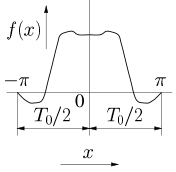
\includegraphics[width=3cm]{Content/Transformationen/gerade_funktion.png}&
        	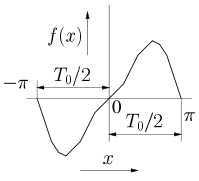
\includegraphics[width=3cm]{Content/Transformationen/ungerade_funktion.png}&   
 			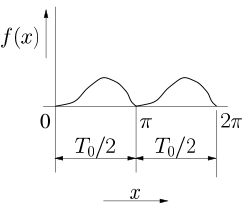
\includegraphics[width=3cm]{Content/Transformationen/halbperiode_1.png}&   
			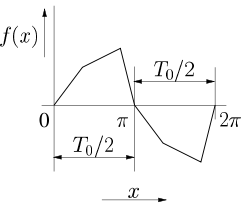
\includegraphics[width=3cm]{Content/Transformationen/halbperiode_2.png}\\
			\hline & & & \\			
   			$f(-t)=f(t)$ & $f(-t)=-f(t)$ & $f(t)=f(t+\pi)$ & $f(t)=-f(t+\pi)$\\
   			$b_k=0$ & $a_k=0$ & $a_{2k+1}=0$ & $a_{2k}=0$\\
   			$a_k = \frac{4}{T} \int\limits_0^{\frac{T}{2}} f(t) \cdot \cos(k \omega_f
   			t) dt$ &
   			$b_k =  \frac{4}{T} \int\limits_0^{\frac{T}{2}} f(t) \cdot
			\sin(k \omega_f t) dt$ &
			$b_{2k+1}=0$ & $b_{2k}=0$\\
			\hline
      	\end{tabular} 
     	
   \subsection{Spektern}
   	\begin{tabular}{p{6cm} p{6cm} p{6cm}}
   		Kosinus- Sinusamplitudenspektrum & 
   		Einseitiges Amplituden-/ Phasenspek. &
   		Zweiseitges Amplituden-/ Phasenspek. \\
   		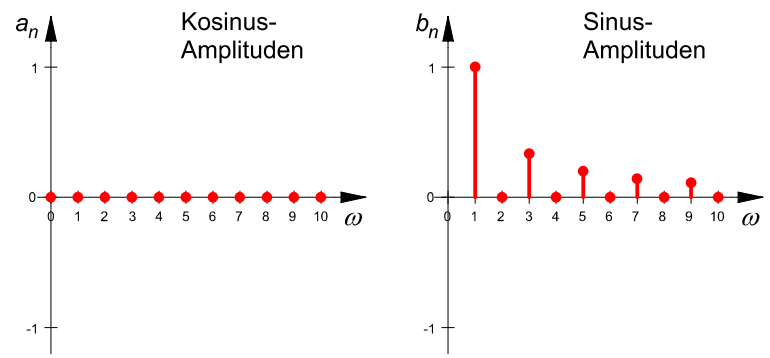
\includegraphics[width=5cm]{Content/Transformationen/cosSinSpectr.png} &
   		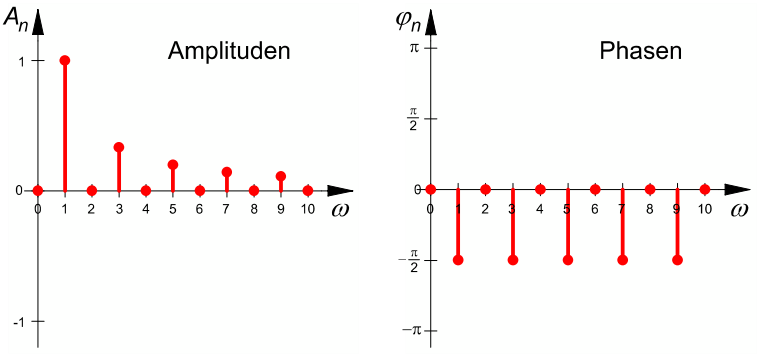
\includegraphics[width=5cm]{Content/Transformationen/EinseitigSpectr.png} &
   		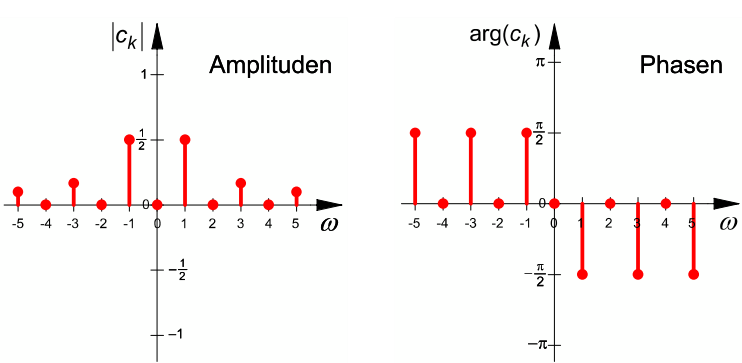
\includegraphics[width=5cm]{Content/Transformationen/ZweiseitigSpectr.png}
   	\end{tabular}
   	Das einseitige und zweiseitige Spektrum unterscheiden sich nur im
  	Amplitudendiagramm. Das Phasendiagramm f"ur positive $k$ ist identisch. Die
  	Amplidudenwerte sind h"alftig auf die pos. und neg. $k$ verteilt.
 